%%%%%%%%%%%%%%%%%%%%%%%%%%%%%%%%%%%%%%%%%%%%%%%%%%%%%%%%%%%%%%%%%%%%%%%%%%%%%%%%
%%%%%%%%%%%%%%%%%%   Vorlage für eine Abschlussarbeit   %%%%%%%%%%%%%%%%%%%%%%%%
%%%%%%%%%%%%%%%%%%%%%%%%%%%%%%%%%%%%%%%%%%%%%%%%%%%%%%%%%%%%%%%%%%%%%%%%%%%%%%%%

% Erstellt von Maximilian Nöthe, <maximilian.noethe@tu-dortmund.de>
% ausgelegt für lualatex und Biblatex mit biber

% Kompilieren mit
% lualatex dateiname.tex
% biber dateiname.bcf
% lualatex dateiname.tex
% lualatex dateiname.tex
% oder einfach mit:
% make

\documentclass[
  tucolor,
  BCOR=12mm,     % 12mm binding corrections, adjust to fit your binding
  parskip=half,  % new paragraphs start with half line vertical space
  open=any,      % chapters start on both odd and even pages
  cleardoublepage=plain,  % no header/footer on blank pages
]{tudothesis}


% Warning, if another latex run is needed
\usepackage[aux]{rerunfilecheck}

% just list chapters and sections in the toc, not subsections or smaller
\setcounter{tocdepth}{1}

%------------------------------------------------------------------------------
%------------------------------ Sprache und Schrift: --------------------------
%------------------------------------------------------------------------------
\usepackage{fontspec}
\defaultfontfeatures{Ligatures=TeX}  % -- becomes en-dash etc.

% german language
\usepackage{polyglossia}
\setdefaultlanguage{german}

% for english abstract and english titles in the toc
\setotherlanguages{english}

% intelligent quotation marks, language and nesting sensitive
\usepackage[autostyle]{csquotes}

% microtypographical features, makes the text look nicer on the small scale
\usepackage{microtype}

%------------------------------------------------------------------------------
%------------------------ Für die Matheumgebung--------------------------------
%------------------------------------------------------------------------------

\usepackage{amsmath}
\usepackage{amssymb}
\usepackage{mathtools}

% Enable Unicode-Math and follow the ISO-Standards for typesetting math
\usepackage[
  math-style=ISO,
  bold-style=ISO,
  sans-style=italic,
  nabla=upright,
  partial=upright,
]{unicode-math}
\setmathfont{Latin Modern Math}

% nice, small fracs for the text with \sfrac{}{}
\usepackage{xfrac}


%------------------------------------------------------------------------------
%---------------------------- Numbers and Units -------------------------------
%------------------------------------------------------------------------------

\usepackage[
  locale=DE,
  separate-uncertainty=true,
  per-mode=symbol-or-fraction,
  binary-units=true
]{siunitx}
\sisetup{math-micro=\text{µ},text-micro=µ}

%------------------------------------------------------------------------------
%-------------------------------- tables  -------------------------------------
%------------------------------------------------------------------------------

\usepackage{booktabs}       % stellt \toprule, \midrule, \bottomrule

%------------------------------------------------------------------------------
%-------------------------------- graphics -------------------------------------
%------------------------------------------------------------------------------

\usepackage{graphicx}
\usepackage{grffile}

% allow figures to be placed in the running text by default:
\usepackage{scrhack}
\usepackage{float}
\floatplacement{figure}{htbp}
\floatplacement{table}{htbp}

% keep figures and tables in the section
\usepackage[section, below]{placeins}


%------------------------------------------------------------------------------
%---------------------- customize list environments ---------------------------
%------------------------------------------------------------------------------

\usepackage{enumitem}

%------------------------------------------------------------------------------
%------------------------------ Bibliographie ---------------------------------
%------------------------------------------------------------------------------

\usepackage[
  backend=biber,   % use modern biber backend
  autolang=hyphen, % load hyphenation rules for if language of bibentry is not
                   % german, has to be loaded with \setotherlanguages
                   % in the references.bib use langid={en} for english sources
]{biblatex}
\addbibresource{references.bib}  % die Bibliographie einbinden
\DefineBibliographyStrings{german}{andothers = {{et\,al\adddot}}}

%------------------------------------------------------------------------------
%------------------------------ Sonstiges: ------------------------------------
%------------------------------------------------------------------------------

\usepackage[pdfusetitle,unicode,linkbordercolor=tugreen]{hyperref}

\AtBeginDocument{%
\newcaptionname{ngerman}{\figureautorefname}{Abbildung}
\newcaptionname{ngerman}{\tableautorefname}{Tabelle}
\newcaptionname{ngerman}{\sectionautorefname}{Kapitel}
\newcaptionname{ngerman}{\chapterautorefname}{Kapitel}%
}

\usepackage{bookmark}
\usepackage[shortcuts]{extdash}

%------------------------------------------------------------------------------
%-------------------------    Angaben zur Arbeit   ----------------------------
%------------------------------------------------------------------------------

\author{Lars Möllerherm}
\title{\LaTeX-Dokumentenklasse und Vorlage für Abschlussarbeiten an der TU Dortmund}
\date{2014}
\birthplace{Mettingen}
\chair{Lehrstuhl für Experimentelle Physik V}
\division{Fakultät Physik}
\thesisclass{Bachelor of Science}
\submissiondate{31. September 2015}
\firstcorrector{Prof.~Dr.~Erstgutachter}
\secondcorrector{Prof.~Dr.~Zweitgutachter}

% tu logo on top of the titlepage
\titlehead{
\includegraphics[height=1.5cm]{logos/tu-logo.pdf}}

\begin{document}
\frontmatter
\maketitle

% Gutachterseite
\makecorrectorpage

% hier beginnt der Vorspann, nummeriert in römischen Zahlen
\thispagestyle{plain}

\section*{Kurzfassung}
In dieser Arbeit wird die Energierekonstruktion von hochenergetischen kosmischen Photonen, welche durch das Cherenkov Telescope Array(CTA) beobachtet
werden, optimiert.
Bisher wird für jedes Teleskop eine eigenständige Energieschätzung durch Algorithmen des überwachten maschinellen Lernens durchgeführt.
Da bei CTA die Möglichkeit besteht, dass mehrere Teleskope den selben Schauer messen, wird durch das Zusammenfassen der einzelnen Ergebnisse die
Energieschätzung verbessert.
Eine einfache oder gewichtete Mittelung über die Schätzungen liefert keinen Qualitätsgewinn, eine verschachtelte und eventspezifische Regression jedoch
führt auf eine Verringerung des relativen Fehlers und auf eine Verbesserung der Energieauflösung.
Der große Zielbereich der Analyse führt auf einen Qualitätsverlust bei niedrigen Energien, was durch eine geeignete bijektive Transformation
geändert wird, wodurch die Schätzung in diesem Energiebereich verbessert werden kann.
Die getesteten Methoden führen auf eine Verringerung des relativen Fehlers und der Energieauflösung um $\SI{75}{\percent}$ in weiten Teilen des Sensitivitätsbereichs von CTA.

\section*{Abstract}
\begin{english}
In this thesis, a method for the optimization of the energy reconstruction for high energy cosmic photons, which are detected by the Cherenkov Telescope Array will be tested.
Currently there is a prediction by supervised machine learning regressors for every single telescope.
Because of the array structure of CTA, the analysis can be optimized by summarizing the results of these telescopes.
There is no performance gain in the simple or the weighted average over each prediction, but a nested model, which predicts every event, causes an improvement
of the relative error and for the energy resolution of CTA.
Because of the estimator´s wide number range, there is a large performance loss for low energies.
This can be managed by a transformation of the output, which ensures a performance improvement.
These methods improve the bias of the relative error and the energy resolution by $\SI{75}{\percent}$ in a large energy range of CTA.
\end{english}

\tableofcontents

\mainmatter
% Hier beginnt der Inhalt mit Seite 1 in arabischen Ziffern
\chapter{Einleitung}

Auf die Erdatmosphäre trifft eine große Menge von hochenergetischer kosmischer Strahlung, welche uns viel über unverstandene
Prozesse im Universum verrät.
Die Gammastrahlung gelangt auf direktem Weg zur Erde, wodurch ihr Entstehungsort erfasst werden kann.
Die Energie der Strahlung liegt weit über der bisher erreichten Schwerpunktsenergie des LHC von ca. $\SI{13}{\tera\eV}$~\cite{LHC} und weckt
ein besonderes Interesse an der Entdeckung neuer Physik.
Als Beispiel dient die Suche nach Zerfällen der Dunklen Materie oder die Untersuchung der physikalischen Gesetze in extremer Umgebung.
Auch ein Großteil der Beschleunigungsprozesse von Teilchen im Universum sind noch nicht erklärt.
Um diese Fragen zu beantworten, muss die Gammastrahlung kosmischer Quellen genau untersucht werden.

Da CTA jährlich $\SI{3.7}{\peta\byte}$~\cite{Rohdaten} an Rohdaten verarbeiten muss, wird eine computergesteuerte Datenanalyse
genutzt und das Feld des maschinellen Lernens liefert die richtigen Werkzeuge.
Eine direkte Beobachtung mithilfe von Satelliten erlaubt es nicht genügend Ereignisse der hochenergetischen Strahlung zu beobachten.
Um eine ausreichende Fläche zu beobachten, wird eine indirekte, erdgebundene Beobachtung über das atmosphärische Schauer und das
entstehende Cherenkov-Licht gewählt.
Diese Lichtblitze werden mithilfe von Cherenkov-Teleskopen gemessen oder im Fall von CTA mit einer Gruppe von Teleskopen.

Um die Ursprungsenergie des Photons zu ermitteln, muss sie mithilfe von Random Forest Regressoren rekonstruiert werden.
Diese Random Forest Algorithmen gehören zum Bereich des überwachten maschinellen Lernens und können mithilfe von Trainingsdatensätzen,
die in Monte-Carlo-Simulationen entstehen, trainiert werden.

CTA besitzt mehr als $\num{100}$ Cherenkov-Teleskope, wobei mehrere Teleskope das selbe Schauer sehen können, jedoch wird momentan für jedes Teleskop eine eigenständige
Energierekonstruktion durchgeführt.
Da jedes Schauer nur ein Primärteilchen besitzt, müssen die Ergebnisse der einzelnen Teleskope zusammengefasst werden oder
eine Schätzung für jedes Schauerereignis und nicht für jedes Teleskop durchgeführt werden.
Da der Sensitivitätsbereich von CTA über vier Größenordnungen geht, könnte eine Transformation diesen Zielbereich verkleinern und
damit dem Random Forest die Schätzung erleichtern.

\chapter{Theoretische Grundlagen}

Um die Performance der Energieschätzung zu verbessern, muss verstanden werden, welche Anforderungen an die Analyse gestellt
werden, um zu neuen Erkenntnissen in der Astroteilchenphysik zu gelangen.
Außerdem muss der Algorithmus des Random Forest genau verstanden werden, um Möglichkeiten des Performancegewinns zu erarbeiten,
wobei am Ende eine sinnvolle Evaluierung der Performance vorgenommen wird.

\section{Gammaastronomie}
\label{sec:Gammaastronomie}

Im Universum gibt es zahlreiche Prozesse, bei denen hochenergetische Teilchen entstehen, oder auf hohe Energien beschleunigt werden.
Bei diesen Teilchen handelt es sich zum großen Teil um Protonen oder leichten Atomkernen bis hin zu Eisenkernen, aber auch Elektronen oder Myonen
sind Bestandteil der kosmischen Strahlung.
Ein großer Teil der Beschleunigung geschieht in Druckwellen, wie sie bei Sternexplosionen vorkommen, dabei spielt das Modell der
Fermi-Beschleunigung erster und zweiter Ordnung eine große Rolle.
%Bei der Fermi-Beschleunigung wird das Medium, indem die Druckwelle propagiert, durch ein Plasma beschrieben, welches Magnetfeldstörungen mit sich führt.
%Wenn ein geladenes Teilchen auf eine solche Störung, welche sich mit einer Geschwindigkeit $v$ durch das Medium bewegt, trifft, wird es durch die
%Lorentzkraft mit einem Winkel $\theta$ elastisch gestreut.
%Wenn nun alle möglichen Winkel berücksichtigt werden, ergibt sich eine Energiegewinn von
%\begin{equation*}
%  \left\langle \frac{\delta E}{E} \right\rangle = \frac{8}{2}\left(\frac{v}{c}\right)^2\text{ .}
%\end{equation*}
%Bei einer typischen Druckwellengeschwindigkeit von $v=\SI{e4}{\m\per\s}$~\cite[14]{HESS} ergibt sich ein Energiegewinn von $\SI{4.5e-9}{\m\per\s}$.
%Dies wird Fermibeschleunigung zweiter Art genannt und kann die große Beschleunigung in Supernovae nicht alleine erklären.
%
%Ein größeren Beitrag liefert die Fermibeschleunigung erster Art, bei der die Teilchen durch mehrfaches durchqueren der Schockfront beschleunigt werden.
%Der Energiegewinn beträgt für alle Streuwinkel
%\begin{equation*}
%  \left\langle \frac{\delta E}{E} \right\rangle \approx \frac{2}{3}\frac{\delta v}{c} \text{ ,}
%\end{equation*}
%wobei $\delta v$ der Geschwindigkeitsunterschied zwischen der Materie hinter und vor der Schockwelle ist.

Für den Teilchenfluss der kosmischen Strahlung direkt nach der Fermibeschleunigung in Schockfronten gilt
$\Phi(E)\approx E^{-2}$.
Wenn die Strahlung mit dem extragalaktischen Plasma wechselwirkt, wird das Spektrum um $E^{-\frac{1}{3}}$ steiler.
Da es auch das Plasma der Milchstraße durchqueren muss, um im Sonnensystem gemessen werden zu können, wird
der Teilchenfluss der kosmischen Strahlung durch $\Phi(E) \approx E^{-2.7}$~\cite[5]{Cosmic_rays} beschrieben.

Jedoch erklären diese Prozesse nicht den gemessenen Energiefluss von ultrahochenergetischen Teilchen, denn bei Energien von $\SI{3e15}{\eV}$ tritt ein erstes
\enquote{knee} im Spektrum auf, welches nicht durch die Fermibeschleunigung erklärt wird.
Die Phänomene die Materie bis auf diese Energien beschleunigen, sind noch nicht vollständig erforscht.
Ein möglicher Prozess wäre die Beschleunigung durch elektrische Potentialunterschiede oder der Zerfall von Dunkler Materie.

Diese hochenergetische Teilchenstrahlung erzeugt durch Wechselwirkungen oder Zerfälle Gammastrahlung.
Wichtige Prozesse bei der Erzeugung hochenergetischer Photonen sind die Wechselwirkungen von Photonen und Elektronen, wie
die inverse Comptonstreuung, wobei das geladene Teilchen Energie auf das Photon
überträgt. Aber auch die Annihilation, welche den Umkehrprozess der Paarerzeugung darstellt und aus einem Elektron Positron Paar
ein Photon erzeugt, und die Bremsstrahlung, bei der ein Photon bei der Impulsänderung geladener Teilchen abgestrahlt wird, spielen eine Rolle.

\begin{figure}
  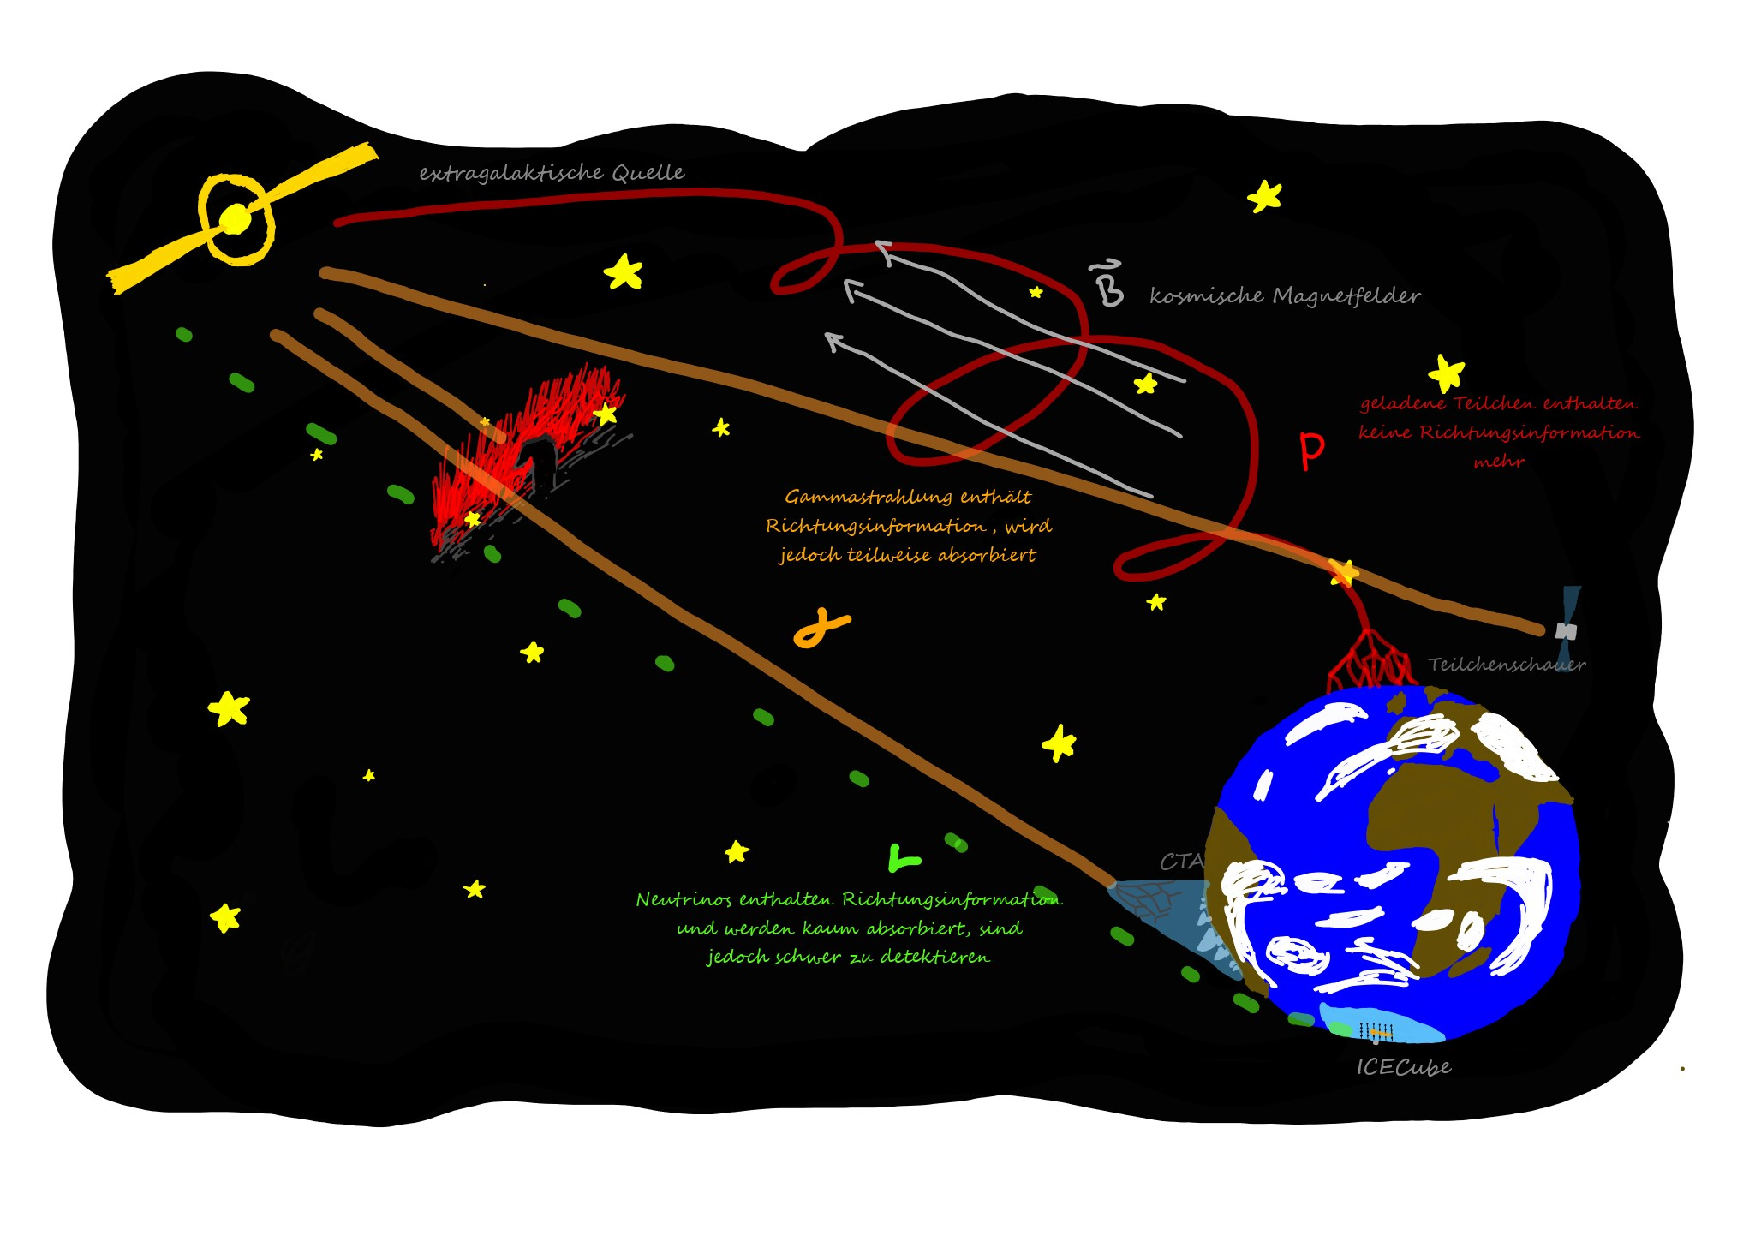
\includegraphics[width=\textwidth]{Plots/Folie5.pdf}
  \centering
  \caption{Skizzierter Weg der kosmischen Strahlung zur Erde. Die Gamma- und Neutrinostrahlung gelangt auf direktem Weg zur Erde, im Gegensatz
            zur geladenen Teilchenstrahlung, die durch kosmische Magnetfelder abgelenkt werden. Die Gammastrahlung wird durch Gaswolken teilweise
            absorbiert. Die Neutrinostrahlung ist jedoch schwer zu detektieren.}
  \label{abb:Folie5}
\end{figure}

\autoref{abb:Folie5} stellt den Weg der kosmischen Strahlung zur Erde dar, wobei die Photonen nicht mit kosmischen Magnetfeldern wechselwirken
und somit deren Ursprungsrichtung bekannt ist. Jedoch wechselwirken die Photonen mit interstellarem Staub, der zwischen der Erde und der
Quelle ist, wodurch ein Teil der Gammastrahlung nicht zur Erde gelangt.

Diese hochenergetischen Photonen können entweder mithilfe von Satelliten im Weltraum oder mithilfe von Cherenkov Teleskopen auf
der Erdoberfläche beobachtet werden.
Aufgrund der hohen Energien der Gammastrahlung können Satelliten diese nur mithilfe von Szintillationszählern messen und nicht durch Spiegelteleskope,
da diese hohen Frequenzen nicht gespiegelt werden, sondern durch die Spiegeloberfläche transmittieren.
Diese energiereiche Strahlung sorgt jedoch dafür, dass in der Erdatmosphäre durch die Wechselwirkung mit den Luftmolekülen ein hochrelativistisches
Teilchenschauer aus überlichtschnellen geladenen Teilchen entsteht.
Da sich bei Geschwindigkeiten über der Lichtgeschwindigkeit des Mediums die durch die Polarisierung entstandenen elektromagnetischen Wellen
nicht mehr destruktiv überlagern, entstehen Cherenkov-Blitze mit einer Dauer von ca. $\SI{150}{\nano\s}$~\cite{Cherenkov_Licht}, welche sich kegelförmig
mit einem Winkel von
\begin{equation}
 \cos(\theta) = \frac{1}{n\beta}
\end{equation}
ausbreiten und von den Cherenkov
Teleskopen am Boden beobachtet werden können.
Der Winkel $\theta$ hängt von dem Brechungsindex $n$ der Luft ab, welcher von der Feuchtigkeit und Dichte der Luft abhängt und somit höhenabhängig ist.
Das kontinuierliche Spektrum der Cherenkov-Strahlung besitzt eine zur Frequenz proportionale Intensität im sichtbaren Bereich und
wird daher als bläulich wahrgenommen.
Die Kamera des Teleskops löst aus, wenn eine bestimmte Anzahl an Photonen des Schauers registriert werden, und nimmt
für eine Dauer von $(150-300)\si{\nano\s}$ Bildmaterial auf.
Da sowohl hochenergetische Gammastrahlung als auch Teilchenstrahlung
Schauer in der Atmosphäre erzeugen, gibt es einen Untergrund, der separiert werden muss.

\section{Cherenkov Teleskope Array (CTA)}
\label{sec:CTA}

Das geplante Cherenkov Teleskop Array wird von einer internationalen Kollaboration von 210 Instituten aus 32 Ländern~\cite{CTA_consortium} geführt
und bildet den nächsten Schritt in der Hochenergiegammaastronomie.
Mit einer Gesamtanzahl von 108 Teleskopen hat das Array nach Simulationen zur Folge in seinem Hauptenergiebereich eine Sensitivität von $\SI{0.1}{\percent}$
des Energieflusses des Krebsnebels, wodurch es ungefähr zehn Mal sensitiver als das HESS-Experiment ist~\cite{CTA_paper}.
Da der Teilchenfluss $\Phi$ der kosmischen Strahlung dem Potenzgesetz $\Phi \propto E^{-2.7}$~\cite[5]{Cosmic_rays} folgt,
treffen bei einer Energie $E$ von $\SI{1}{\tera\eV}$ noch $\SI{1}{\per\m\squared\per\s}$ Teilchen auf die Erdatmosphäre.
Um dennoch genug Statistik zu besitzen, muss eine möglichst große Himmelsfläche observiert werden.
Durch die große Anzahl an Teleskopen kann CTA mit einer diverged mode Beobachtung eine Himmelsfläche von $\SI{20}{\degree}\times \SI{20}{\degree}$
beobachten~\cite[16]{CTAscience}.
Durch drei verschiedene Teleskopgrößen kann CTA Photonen mit Energien von $\SI{30}{\giga\eV}$ bis $\SI{300}{\tera\eV}$ detektieren,
was es ermöglicht, die verschiedenen Beschleunigungsprozesse im Universum zu untersuchen.
Insbesondere kann das \enquote{knee} bei $\SI{3e15}{\eV}$ genauer untersucht werden.
Zu den Arten gehören das LST (Large Sized Telescope) mit einer Spiegelgröße von $\SI{23}{\m}$, das MST (Medium Sized Telescope)
mit einer Größe von $\SI{11.5}{\m}$ oder $\SI{9.7}{\m}$ und das SST (Small-Sized Telescope), welches eine Größe von $\SI{4.3}{\m}$ oder $\SI{4.0}{\m}$
besitzt~\cite{CTA_tec} .
Die hohe Sensitivität und die niedrige Energieuntergrenze ermöglichen die Entdeckung neuer Quellen mit einer starken Rotverschiebung, die nur bei niedrigen
Energien sichtbar sind, da die höherenergetische Gammastrahlung mit der Hintergrundstrahlung wechselwirkt und somit nicht beobachtet werden kann.
Die große Anzahl an Teleskopen führt zusätzlich auf eine bessere Winkelauflösung, was entscheidend bei der Multimessenger Beobachtung von Quellen ist, welche
durch die ersten Neutrinoquellen Identifizierung im Jahr $2018$ ~\cite{IceCubeobs} immer vielseitiger und erfolgreicher wird.

\section{Maschinelles Lernen}
\label{sec:ML}

Aufgrund des geringen Teilchenflusses bei hohen Energien, muss die Anzahl an beobachteten Ereignissen bei modernen
Experimenten stark ansteigen, wodurch eine händische Analyse unmöglich wird.
Daher werden Algorithmen des maschinellen Lernens trainiert, die diese Aufgabe übernehmen.
Das maschinelle Lernen wird als Teilgebiet der künstlichen Intelligenz verstanden. Hierbei lernen Algorithmen aus Datensätzen,
indem sie verschiedene Optimierungsverfahren nutzen, um eine Fehlerfunktion zu minimieren.
Ein trainierter Algorithmus kann im Anschluss Vorhersagen über neue Datenpunkte treffen.

Der Bereich des maschinellen Lernens wird in das überwachte Lernen, bei dem das Ergebnis und die Eingangsdaten bekannt
sind und das unüberwachte Lernen, bei dem der Algorithmus Muster in den Eingangsdaten sucht, gegliedert.
Zwei große Aufgabengebiete im Bereich des überwachten Lernens sind die Regression und die Klassifikation. Die Regression bildet
auf die reellen Zahlen ab und die Klassifikation auf $N$ Klassen, womit die Regression als Grenzfall $N \to \infty$ der Klassifikation
verstanden werden kann.

Das Modell der Regressionsanalyse benutzt die abhängige Variable $y$ die über eine Funktion $f(X,\theta)$ von der Variable $X$ abhängt, um
den Parameter $\theta$ so zu optimieren, dass für $\hat{y} = f(X,\theta) + L(\hat{y},y)$ der Fehler
$L(\hat{y},y)$ minimiert wird.
Wenn $\vec{\theta}$ aus k Parametern besteht und $(X_i,y_i)$ $N$ Tupel sind, müssen drei Fälle unterschieden werden.
Im ersten Fall gilt $k>N$, was zu einem unterbestimmten System führt, in dem es nicht genug Datenpunkte gibt, um alle Parameter
vorherzusagen, wodurch viele Regressionsmethoden zu keinem Ergebnis führen.
Bei $k = N$ existiert genug Information um ein lineares System exakt zu lösen.
Im letzten Fall gilt $k<N$, was das System überbestimmt werden lässt, wodurch mehreren Lösungen existieren und
es wird die Lösung gewählt, die $L(\hat{y},y)$ minimiert.
Bei der linearen Regression wird angenommen, dass der Trainingsdatensatz das Problem vollständig repräsentiert und $L(\hat{y},y)$ keinen Trend
und keine Korrelation besitzen.
Eine weitere Annahme muss sein, dass, wenn die Variable $X$ einen Vektor darstellt, für diese Unkorreliertheit und lineare Unabhängigkeit gilt.
Wenn der Fehler von $X$ eine nicht konstante Varianz besitzt, muss dies durch eine gewichtete Methode korrigiert werden.

\section{Random Forest Regressor}
\label{sec:RF}

Eine Methode des überwachten Lernens, welche für die Regression verwendet werden kann, stellt der Random Forest Algorithmus dar. Dieser Algorithmus baut
einen Wald aus mehreren unkorrelierten Entscheidungsbäumen auf, die eigenständige Vorhersagen treffen, über die abschließend gemittelt wird.

Ein Entscheidungsbaum wird aufgebaut, indem der Datensatz in Teildatensätze aufgeteilt wird, wobei ein gewähltes Kriterium optimiert wird.
Dieses Kriterium
kann die Gini Unreinheit oder der Informationsgewinn sein, bei der Regression wird jedoch häufig die Varianzreduktion verwendet.
Bei dieser Optimierung wird in jedem Schritt der mittlere quadratische Fehler
\begin{equation}
  H(X_m) = \frac{1}{N_m}\sum_{i\in N_m}(y_i-c_m)^2
\end{equation}
jedes Teildatensatzes $m$ minimiert, mit
\begin{equation}
  c_m = \frac{1}{N_m}\sum_{i\in N_m}\hat{y}_i
\end{equation}
als Mittelwert der Vorhersage $\hat{y}_i$ für jeden Datenpunkt $i$ und $y_i$ als wahren Wert.
Dies wird rekursiv wiederholt und somit der Baum ausgebaut, bis der Algorithmus ein Abbruchkriterium erfüllt.
Dieses Abbruchkriterium kann eine vorher festgelegte maximale Tiefe
des Baumes sein, eine minimale Größe des Datensatzes, der getrennt werden soll, oder eine minimale Größe des getrennten Datensatzes. Nach Erreichen der Abbruchbedingung bildet
$c_m$ des letzten Schrittes die endgültige Vorhersage.

Bei Entscheidungsbäumen gibt es eine Vielzahl von Umsetzungen.
Die aktuellsten Arten sind der C5.0 und der CART Algorithmus~\cite[1]{CART}.
Die Besonderheit am C5.0 Algorithmus stellt, im Gegensatz zum CART Algorithmus, die nicht notwendige binäre Trennung des Datensatzes dar,
jedoch kann mit ihm keine Regression durchgeführt werden.
Im \textsc{scikit-learn}-Framework~\cite{scikit-learn} wird eine CART Implementierung des Entscheidungsbaumes benutzt, welche zur
Regression fähig ist und die Varianzreduktion als Optimierungskriterium nutzt.

Die Vorteile eines Entscheidungsbaumes sind die Interpretierbarkeit, die Zeitkomplexität von $\Omega(n\log(n))$ bei $n$ Datenpunkten und die einfache Datenpräparation.
Außerdem besteht keine Anfälligkeit gegenüber unbedeutenden Attributen.
Jedoch besteht eine Gefahr des Übertrainierens, was bei einem zu großen Ausbauen des Baumes dazu führt, dass der Trainingsdatensatz nachgebildet
wird und die Vorhersagen für einen unabhängigen Testdatensatz unpräzise werden.
Des Weiteren kann es zu einer Verzerrung in den Vorhersagen kommen, wenn der Trainingsdatensatz eine Verzerrung aufweist.
Entscheidungsbäume besitzen keine Stabilität gegenüber Änderungen im Datensatz, was zu einer hohen Varianz der Ergebnisse
unterschiedlicher Bäume führt.
Da der Entscheidungsbaum zu den gierigen Algorithmen gehört, welche die Entscheidung aufgrund des derzeitig besten Gewinns treffen, findet dieses Verfahren schnell ein
Optimum, jedoch nicht immer das globale Extremum und somit nicht die optimale Lösung.
Die letzten beiden Nachteile können durch die Erweiterung des Entscheidungsbaumes zu einem Entscheidungswald behoben werden.

Dieses Verfahren wird Random Forest (RF) genannt. Beim RF werden eine Vielzahl von Entscheidungsbäumen, um Unkorreliertheit der Ergebnisse zu erreichen, mit
zufällig ausgewählten Teildatensätzen und Attribute trainiert. Das Ergebnis des RF ergibt sich durch eine Mittelung über alle Entscheidungsbäume.
Wenn die Anzahl der Entscheidungsbäume erhöht wird, konvergiert der generalisierte Fehler
\begin{equation}
  PE = P_{X,y}(mg(X,y)<0)
\end{equation}
gegen
\begin{equation}
  P_{X,y}(P_\theta(h(X,\theta)=y)-\max_{j\neq y}P_\theta(h(X,\theta)=j)<0)
\end{equation}
und es kann durch eine Vergrößerung des Waldes nicht zum Übertraining kommen~\cite[7]{RandomForests_Breiman}. Bei diesem Theorem bildet
\begin{equation}
  mg(X,y) = av_k I(h_k(X)=y) - \max_{j \neq y}av_k I(h_k(X)=j)
\end{equation}
die Gewinn Funktion, $h_k(X)$ die Vorhersage der $k$ Entscheidungsbäume und $I(\cdot)$ die charakteristische Funktion, welche eine $1$ ergibt, wenn der
Entscheidungsbaum das geforderte Ergebnis liefert und eine $0$ wenn nicht.
Wenn $mg(X,y) > 0$ gilt, sagt der Entscheidungsbaum das richtige Ergebnis vorher.

Um einen unkorrelierten Wald zu erhalten, muss die Auswahl der Teildatensätze und der Attribute zufällig und unabhängig getroffen werden.
Dazu kann unter anderem das Adaboost Verfahren oder das Bagging verwendet werden.
Dass in \textsc{scikit-learn} verwendete Bagging funktioniert, indem aus dem Datensatz $N$ Stichproben der Größe $M$ gezogen werden und für die $N$ Entscheidungsbäume verwendet werden.
Die $N$ Ergebnisse werden am Ende gemittelt oder zusätzlich mit der Genauigkeit des jeweiligen Ergebnisses gewichtet.
Um die Größe der Datensätze nicht zu verkleinern, ist es möglich die Datensätze mit Bootstrapping künstlich zu vergrößern, wobei Datenpunkte durch andere Datenpunkte
des Datensatzes zufällig ersetzt werden, anstatt sie zufällig auszusortieren.
Zusätzlich zum Bagging werden bei einem RF die Attribute in einem Umfang, der festgelegt werden kann, zufällig gezogen.
Hierdurch verlieren die Entscheidungsbäume an Genauigkeit, die Korrelation des Ergebnisses verringert sich jedoch,
was Verzerrung-Varianz-Dilemma genannt wird. Die Varianz wird soweit minimiert, dass es zu keiner Überanpassung kommt
und die Verzerrung möglichst klein bleibt~\cite[2]{Hyperparameter_RF}.

Durch Kreuzvalidierung kann das Modell auf Übertraining untersucht werden. Hierbei wird der Datensatz aufgeteilt, um
den Algorithmus mit einem Teil zu trainieren und mit dem anderen unabhängigen Teil zu testen.
Die einfache Kreuzvalidierung stellt die in \textsc{scikit-learn} implementierte Methode dar, bei der der Datensatz
in $k$ Teildatensätze geteilt wird und jeder dieser Datensätze einmal als Validierungsdatensatz
verwendet wird und $k-1$ Datensätze zum Training dienen.

\section{Energie Rekonstruktion}

Um die in \autoref{sec:Gammaastronomie} erwähnten Bilder auszuwerten, muss zunächst die Kamera kalibriert werden, da die Funktionsweise der elektronischen
Komponenten stark von äußeren Bedingungen beeinflusst wird.
Der nächste Schritt stellt das Extrahieren der wichtigen Information aus dem Kamerabild in Form der Hillasparameter dar.
Dabei wird angenommen, dass die Kamera den Schauer als Ellipse sieht, wobei diese Ellipse eine Länge $L$ und Breite $w$ besitzt.
Weitere Parameter sind die $x$-und $y$- Koordinate des Ellipsenmittelpunkts sowie dessen Polarkoordinaten $r$ und $\phi$ oder der Rotationswinkel $\psi$
der Ellipsenhauptachse, welcher relativ zur Verbindungslinie zwischen Ellipsenmittelpunkt und Kameramittelpunkt gemessen wird.
Die geometrischen Hillasparameter sind in \autoref{abb:Hillas} dargestellt.
\begin{figure}
  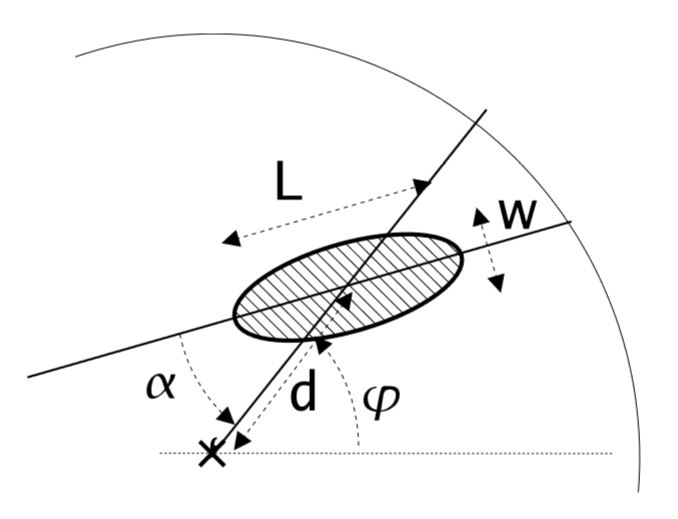
\includegraphics[width=0.5\textwidth]{Plots/Hillas.JPG}
  \centering
  \caption{Schematische Darstellung der Hillasparameter, die das Kamerabild der Schauer charakterisieren. Diese Parameter
            werden verwendet, um die Energie des primären Teilchens zu schätzen.~\cite[101]{HESS}}
  \label{abb:Hillas}
\end{figure}
Ein weiterer wichtiger Parameter bildet die totale Intensität des Bildes und da CTA aus mehreren unterschiedlichen Teleskopen besteht, bekommt die Anzahl
der Teleskope, die den gleichen Schauer gesehen haben, und welche Art von Teleskop dieses Schauer gesehen hat, eine große Bedeutung für die anschließende
Signal Separation und Energie Schätzung.

Diese Parameter werden genutzt um die Untergrundschauer von den photoninduzierten Schauern zu trennen.
Diese Aufgabe wird mit einer Klassifizierungsmethode des maschinellen Lernens gelöst und der
RF Classifier stellt den qualifiziertesten Algorithmus dar.
%Durch das Verhältnis von Signal zu Untergrund von $\approx \frac{1}{1000}$~\cite{Cherenkov_Licht} wird eine große Menge Trainingsdaten
%benötigt, um eine gute Trennung zu ermöglichen.

Nach einer erfolgreichen Separation können diese Parameter genutzt werden, um die Energie des Photons zu schätzen.
Dies kann durch Regressionsmethoden gelöst werden, wobei der RF sich als stabilster Algorithmus erweist~\cite{Cherenkov_Licht}.

Die in \autoref{sec:ML} aufgeführten Annahmen für eine erfolgreiche Regressionsanalyse, sind bei diesem Problem bestmöglich erfüllt. Die Trainingsdaten
werden durch Monte Carlo Simulationen erstellt, die die Wechselwirkung der Primär- und Sekundärteilchen mit der Atmosphäre und die Reaktion des Teleskops
auf das Schauerlicht simuliert.
Dadurch repräsentiert der Trainingsdatensatz das Problem bestmöglich, jedoch führen mögliche systematische Fehler in der Simulation zu einer Verzerrung.
Darüber hinaus werden die Parameter mit der größtmöglichen Präzission gemessen um den Fehler der Parameter zu minimieren,
jedoch sind aufgrund der Berechnung der Hillasparameter, welche in ~\cite[102]{HESS}
genauer beschrieben werden, diese nicht linear unabhängig.
Auch die Varianz des Fehlers geht aufgrund der unterschiedlichen Sensitivitäten der Teleskope nicht homogen
über den ganzen Energiebereich, was jedoch durch eine Gewichtung ausgeglichen werden könnte.

\section{Performance}
\label{sec:Per}

Um zu erkennen, ob das weiterentwickelte Modell eine genauere Vorhersage liefert als das Bisherige, muss die
Performance des RFs beurteilt werden können.

Für einen ersten Überblick über die Genauigkeit des Algorithmus, wird die Wahrheit gegen die Vorhersage in einem
zweidimensionalen Histogramm aufgetragen, welches als Migrationsgrafik bezeichnet wird.
Dabei hat die Diagonale die Bedeutung der genauen Vorhersage und eine geringe Streuung der gefüllten Bins
um diese deutet auf einen guten Schätzer hin.
Die Aussagekraft dieser Abbildung hängt von der Anzahl der Behälter ab, daher wird ein Raster von $300 \times 300$ verwendet.

Ein mögliches Maß, um die Anpassungsgüte von Regressionsmodellen beurteilen zu können, stellt der Determinationskoeffizient dar, welcher
durch
\begin{equation}
  R^2 = 1 - \frac{\sum_i (y_i-\hat{y}_i)^2}{\sum_i (y_i - \overline{y})^2}
\end{equation}
definiert wird. Wobei $\hat{y_i}$ die Schätzwerte, $\overline{y}$ der Mittelwert und $y_i$ die Messwerte darstellen.
Der Determinationskoeffizient nimmt den Wert $1$ an, wenn das Modell die Messpunkte genau beschreibt. Wenn jedoch
$R^2 \leq 0$ ist, kann das Modell als unbrauchbar eingestuft werden, da die Attribute $X$ keine Information zur
Lösung des Problems einbringen.

Dieser Koeffizient besitzt Grenzen der Interpretierbarkeit, da er nur eine Aussage über das gesamte Modell macht und
nicht über die Genauigkeit in einzelnen Wertebereichen.
Außerdem reagiert er empfindlich gegenüber Trends, die $R^2$ senken, obwohl dies nicht bedeutet, dass das Modell die Abhängigkeiten des Problems
nicht gut beschreibt.
Des Weiteren muss die gleiche Anzahl an Datenpunkten vorliegen, um Modelle
miteinander zu vergleichen.

Eine Aussage über die Genauigkeit des Algorithmus kann auch über den relativen Fehler getroffen werden. Dabei spielen der Mittelwert und die
Hälfte des Interquartilen Abstandes (IQA) von $\SI{68.26}{\percent}$, der durch
\begin{equation}
  IQA = \frac{Q_{84}-Q_{16}}{2}
\end{equation}
definiert wird, eine wichtige Rolle.
Dabei stellt $Q_{84}$ das $\SI{84.13}{\percent}$ Quantil und $Q_{15}$ das $\SI{15.87}{\percent}$ Quantil dar, welche durch die \textsc{numpy}-Bibliothek~\cite{scipy}
bestimmt werden, die das $q$-te Quartil als den $q \cdot N$-ten Wert eines geordneten Datensatzes der Größe $N$ definiert.
Der Mittelwert ist ein Maß für die Verzerrung und der IQA ist ein Maß für die Auflösung des Schätzers, wobei dies für unterschiedliche
Energie-Bins untersucht wird, da aufgrund der energieabhängigen Statistik auch diese Werte über das Energiespektrum hinweg variieren.

Ein weiteres Maß stellt der gemittelte quadrierte Fehler
\begin{equation}
  mse = \frac{1}{N} \sum_i (y_i-\hat{y}_i)^2
\end{equation}
dar.
Wenn dieser Fehler kleiner wird, verringert sich auch der relative Fehler, jedoch ist die Größe der Verringerung abhängig vom Energiebereich.
Wie in \autoref{sec:RF} beschrieben, wird der RF anhand dieses Kriteriums minimiert.

Die Frage ob der relative Fehler oder der $mse$ minimiert werden soll, hängt von der angestrebten Analyse ab.
Soll ein Energiespektrum erstellt werden, um ein Potenzgesetz zu analysieren, bietet sich die Minimierung des relativen Fehlers an, da die
Energie logarithmisch aufgetragen wird.
Ist jedoch die Untersuchung eines Linienspektrums, wie bei der Suche nach Zerfällen der Dunklen Materie, die Absicht der Analyse, dann sollte
der absolute Fehler in dem zu analysierenden Energiebereich minimiert werden.


Um die Frage des Informationsgehalts der Attribute zu beantworten, kann zum Beispiel die Wichtigkeit mithilfe von Selektionshäufigkeit, Gini Wichtigkeit oder
die Wichtigkeit der Permutations Genauigkeit bestimmt werden.
Die in \textsc{scikit-learn} implementierte Methode nutzt die Rangordnung der Attribute in den einzelnen Entscheidungsbäumen, indem die früh und häufig genutzten Attribute
als wichtiger klassifiziert werden.
Diese Wichtigkeit kann für jeden Baum ausgelesen werden und als Boxplot dargestellt werden.
Dabei stellt die durchgezogene Linie den Median dar, die Enden des Kastens das $\num{0.25}$-und das $\num{0.75}$-Quartil, die Antennen das $\num{0.125}$-und das
$\num{0.875}$-Quantil und die Punkte stellen Ausreißer, die außerhalb des $\num{0.75}$-IQA liegen, dar.
Wenn eine unterschiedliche Zahl an Kategorien oder ein unterschiedlich großer Wertebereich der Attribute vorliegt, besitzt Bootstrapping mit Ersetzen der Datenpunkte
und die Attribut Selektion bei CART Algorithmen eine Verzerrung, welche sich auf die Bestimmungsmethoden der Wichtigkeit überträgt und somit das Ergebnis verfälschen
kann~\cite{feature_importance}.

\chapter{Ergebnisse}
Aufgrund der Architektur von CTA bietet sich eine Mittelwertbildung über das Array an, um die Qualität des Schätzers zu verbessern.
Zusätzlich scheint aufgrund der Tatsache, dass die Energie des primären Teilchens proportional zur Schauergröße ist und das
ganze Array eine bessere Aussage über die Größe treffen kann als einzelne Teleskope, eine Zusammenfassung der
Information aller Teleskope sinnvoll.
Da das in \autoref{sec:RF} beschriebene Kriterium sich auf den absoluten Fehler und nicht auf den relativen Fehler
bezieht, muss der Tatsache, dass die richtige Schätzung großer Energien für den Algorithmus einen größeren Gewinn bedeutet,
durch Transformationen entgegengesteuert werden, um eine gute Energieauflösung in allen Energiebereichen zu erlangen.

\section{Energierekonstruktion mit Hilfe eines Random Forest Regressors}
\label{sec:first}

Um ein Vergleichsergebnis zu erhalten, wird zunächst ein Random Forest Regressor, wie er in \autoref{sec:RF} beschrieben wird, verwendet,
der eine Energieschätzung für jedes Teleskop vornimmt.
Für das Training werden nur Gamma Ereignisse verwendet und somit eine erfolgreiche Signal-Untergrund Trennung vorausgesetzt.
Für ein realitätstreueres Testen werden diffuse und punktgerichtete Gamma-Simulationsdaten verwendet, da in der
Realität die Signal-Extraktion nicht zwischen punktgerichteten Photonen und Photonen, die in der Atmosphäre entstehen oder zu der
allgemeinen kosmischen Strahlung gehören, unterscheiden kann.

Als Attribute werden die nicht richtungsabhängigen Hillasparameter verwendet, dazu gehören Intensität, Länge, Breite, Schiefe und Wölbung sowie
die totale Intensität, die von allen Teleskopen aufgenommen wird.
Zusätzlich werden die Anzahl der ausgelösten Teleskope, SST, MST und LST als Attribute genutzt, sowie die Identifikationsnummer des
Teleskops, welche für das LST $1$, für das MST $2$ und für das SST $3$ ist.

Des Weiteren werden die skalierte Länge
\begin{equation}
  SW = \frac{w- \langle w \rangle}{\sigma_w}
\end{equation}
und Breite
\begin{equation}
  SL = \frac{l - \langle l \rangle}{\sigma_l}
\end{equation}
verwendet, wobei der Mittelwert über alle Trainingsdatenwerte genommen wird. Diese Methode nennt sich Scaled Cuts Technik.~\cite[104]{HESS}

Der ganze Datensatz besteht aus $\num{3322938}$ Datenpunkten, wovon $\SI{78}{\percent}$ punktgerichtete Photonen und $\SI{22}{\percent}$ diffuse Photonen sind,
die in $\SI{33}{\percent}$ Trainings- und $\SI{66}{\percent}$ Testdatensatz aufgeteilt werden.
Die Aufteilung geschieht jedoch mithilfe der Ereignisnummer, damit bei der Trennung keine Ereignisse getrennt werden.
Diese Datenpunkte stellen Teleskop-Ereignisse dar.
Jedes Schauer stellt ein Array-Ereignis dar, was von mehreren Teleskopen gemessen werden kann und somit mehrere Teleskop-Ereignisse beinhalten kann.

Bei dem Training wird ein Random Forest verwendet, der zur Verhinderung des Übertrainings eine maximale Tiefe von $10$ Ebenen besitzt.
Jeder Baum trainiert mit $\sqrt{N}$ Attributen, wobei $N$ Attribute zur Verfügung stehen, um Korreliertheit der Bäume zu vermeiden,
was zu gleichen Baumstrukturen führen würde und somit zu bevorzugten Ergebnissen.
Außerdem besteht der Wald aus $100$ Bäumen, was mit einer größeren Rechenleistung vergrößert werden kann, ohne
das es, wie in \autoref{sec:RF} erklärt, zum Übertraining kommt.
Der Algorithmus nutzt das Kriterium der Varianz-Reduktion. Da die gering gewählte Tiefe
ein Übertraining bereits verhindert und die Ereigniszahl ausreichend groß ist , werden die Hyperparameter
der minimalen Blatt- und Trenngröße auf ihrer Grundeinstellung von $1$ und $2$ gelassen.

\begin{figure}
  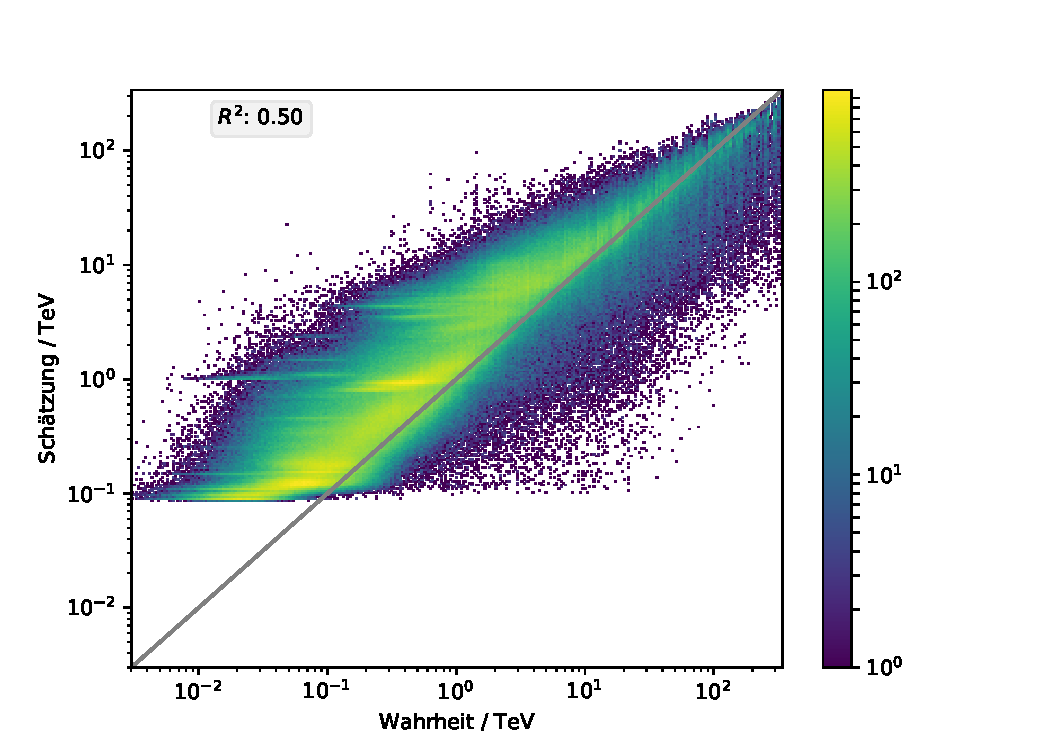
\includegraphics[width=0.7\textwidth]{Plots/RF.pdf}
  \centering
  \caption{In diesem Graphen ist die vorhergesagte Energie gegen die Wahrheit aufgetragen, wobei Streuung und Verzerrung um die
          Diagonale zu erkennen sind.}
  \label{abb:Energie_RF}
\end{figure}
Dieser trainierte Entscheidungswald wird mit $\num{2193140}$ Teleskop-Ereignissen getestet und liefert eine Qualität, wie sie in \autoref{abb:Energie_RF} zu sehen ist.
Dabei ist eine Überschätzung der Wahrheiten zu beobachten sowie feine horizontale Linien, die auf eine Korreliertheit der Entscheidungsbäume hindeuten.
Der $R^2$-Wert von $\num{0.50}$ deutet auf eine bessere Beschreibung des Modells als der bloße Mittelwert hin.
Die Korreliertheit und die Verzerrung können durch eine geeignetere Wahl der Hyperparameter minimiert werden.
Es ist zu betonen, dass durch die Schätzung auf Teleskop-Ereignissen dieser RF mehrere Vorhersagen für das selbe Schauer liefert.

\begin{figure}
  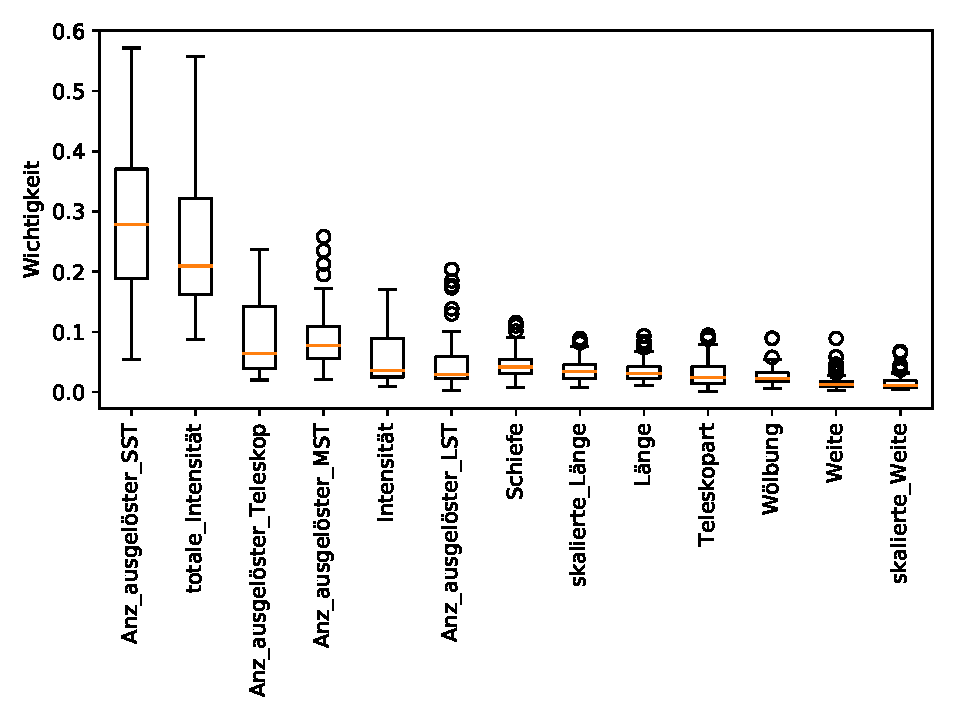
\includegraphics[width=0.7\textwidth]{Plots/feautureimportance_boxplot_firstForest.pdf}
  \centering
  \caption{Darstellung der Wichtigkeit der genutzten Attribute bei der ersten Vorhersage als Kastengrafik. Die Anzahl der ausgelösten SST und die totale Intensität
          stellen die wichtigsten Attribute dar und die Breite der Hillasellipse trägt kaum zur Schätzung bei.}
  \label{abb:first_FI}
\end{figure}
Wie in \autoref{abb:first_FI} dargestellt, besitzen eventspezifische Attribute wie die Anzahl der ausgelösten Teleskope und die totale Intensität die größte Wichtigkeit und teleskopspezifische Attribute
wie die Hillasparameter liefern keinen großen Informationsgewinn.
Eine Erklärung liefert die Tatsache, dass die in dem Schauer deponierte Energie ein wichtiger Parameter für die Energieschätzung ist und die Hillasparameter im
Gegensatz zu den eventspezifischen Parametern von dem Abstand des Teleskops zum Schauer abhängen.
Aufgrund der Unterschiedlichkeit der Attribute kann die Wichtigkeit nach \autoref{sec:Per} eine Verzerrung besitzen und Attribute
wie die Intensität überschätzt, sowie Attribute wie die Teleskopart unterschätzt werden.

\section{Optimierung durch Mittelwerte und geeignete Gewichte}

Um eine physikalisch sinnvolle Aussage über die Energie des Primärteilchens treffen zu können, müssen die Schätzungen der
Teleskop-Ereignisse zusammengefasst werden und somit ein Ergebnis für jedes Array-Ereignis gefunden werden.
Die Energieschätzung der einzelnen Teleskope bei einem Ereignis variiert, obwohl sie den gleichen Schauer beobachten.
Dies liegt an den unterschiedlichen Arten, Blickwinkeln und Abständen der Teleskope, was dazu führt, dass jedes Teleskop unterschiedlich viel Information über den
Schauer erfasst.
Wenn die variierenden Ergebnisse zufällig und nach dem Zentralen Grenzwertsatz der Statistik normalverteilt um den
wahren Wert liegen~\cite[10]{zufall_Fehler}, verbessert eine Mittelwertbildung das Ergebnis.
Daher wird als Schätzer das arithmetische Mittel und der Median untersucht.
\begin{figure}
  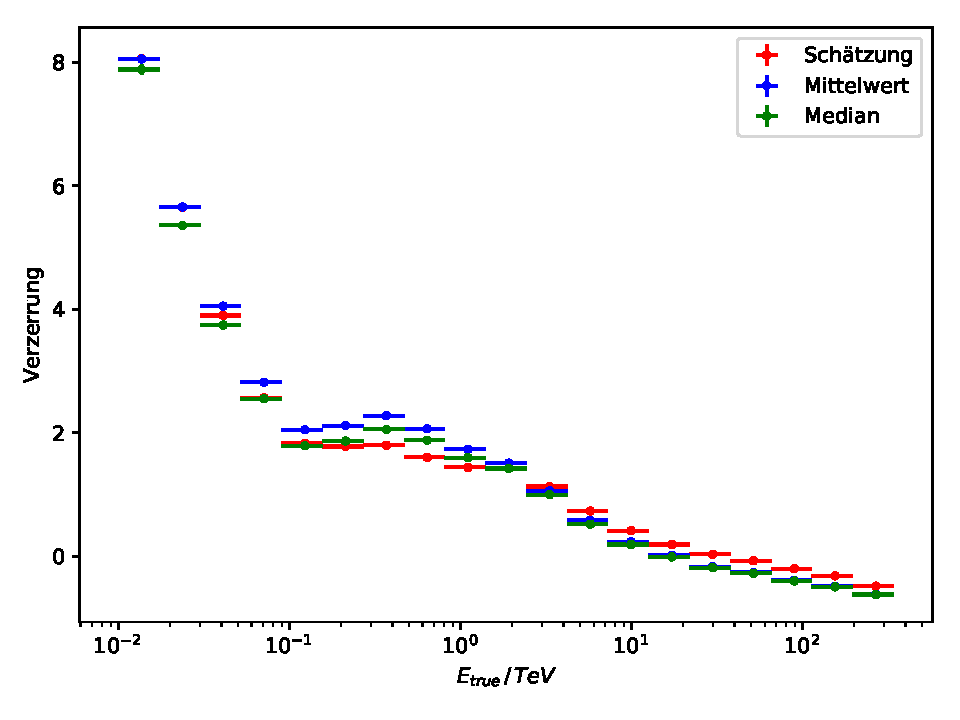
\includegraphics[width=0.7\textwidth]{Plots/RF_mean_bias.pdf}
  \centering
  \caption{Darstellung der Verzerrung für verschiedene Energiebereiche. Es sind die Mittelwerte der relativen Fehler für die Schätzung der Teleskop-Ereignisse, die Vorhersage
          nach der Mittelwertbildung und der Median der Vorhersagen aufgetragen.}
  \label{abb:mean_median_bias}
\end{figure}
\begin{figure}
  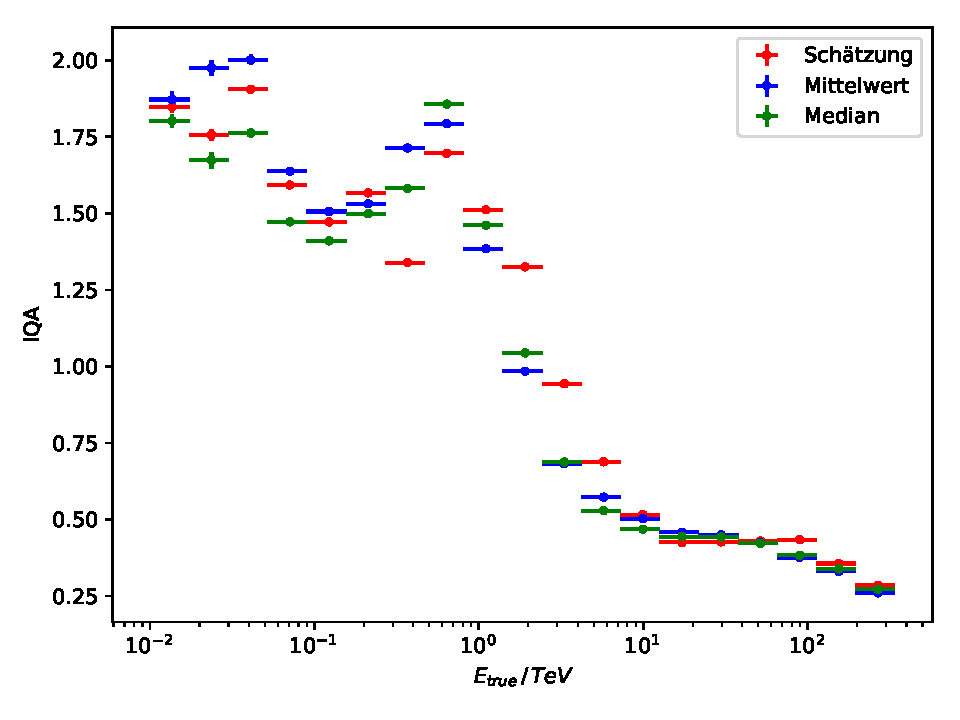
\includegraphics[width=0.7\textwidth]{Plots/RF_mean_resolution.pdf}
  \centering
  \caption{Darstellung des IQA des relativen Fehlers für verschiedene Energiebereiche. Aufgetragen sind die Schätzung der Teleskop-Ereignisse, die Vorhersage
          nach der Mittelwert Bildung und der Median der Vorhersagen.}
  \label{abb:mean_median_IQA}
\end{figure}

Die zusammengefassten Schätzungen führen auf die Verzerrungen und IQAs, die in \autoref{abb:mean_median_bias} und \autoref{abb:mean_median_IQA} zusehen sind.
Bei niedrigen Energien führt das arithmetische Mittel auf keine geringere Verzerrung und auch der Median bringt nur eine leichte Verbesserung.
Dies liegt daran, dass eine Verzerrung die Annahme verletzt, dass die Ergebnisse um den wahren Wert liegen, stattdessen liegen sie um einen verschobenen
Wert.
Das arithmetische Mittel kann eine Verzerrung nicht verringern.
Nur bei Ereignissen mit einer geringen Verzerrung sorgt das Mitteln für eine bessere Qualität, was zum einen bei dem IQA für große Energien zu beobachten
ist und bei dem gesamten gemittelten quadratischen Fehler, der von $\SI{102.94}{\tera\eV\squared}$ für die erste Schätzung auf $\SI{65.31}{\tera\eV\squared}$ nach einer
Mittelwertbildung fällt.

Das der Median die Verzerrung verringert liegt daran, dass es bei dem Beobachten von Schauern vorkommen kann, dass einzelne Teleskope im Gegensatz zu anderen
besser positionierten Teleskopen nur einen geringen Teil des Schauers beobachten und somit weniger Information des Schauers besitzen, was zu einer falsche Vorhersage
führt.
Da dies meist nur auf vereinzelte Teleskope zutrifft, liegt der Median der Teleskope richtig.
Dies zeichnet sich auch durch einen gemittelten quadratischen Fehler von $\SI{66.61}{\tera\eV\squared}$ aus, welcher besser als der Fehler der ersten Schätzung ist und
vergleichbar mit dem Fehler der Mittelwertbildung ist.

Eine weitere Möglichkeit um das Problem, dass nicht alle Teleskope den Schauer gleich gut sehen, zu beheben, stellt das Mitteln mit einem Gewicht, welches die
Sichtbarkeit des Schauers beschreibt, dar.
Ein Indiz auf den gesehenen Anteil des Schauers stellt die beobachtete Intensität dar , wobei eine hohe
Intensität eine gute Sichtbarkeit bedeutet und somit die Intensität direkt als Gewicht verwendet wird.

Zum Anderen besitzen die in \autoref{sec:CTA} beschriebenen Teleskope eine energieabhängige Sensitivität, wobei
es einen Energiebereich gibt, indem eine volle Sensitivität herrscht und einen, indem eine Teilsensitivität
herrscht.
Das LST besitzt eine Teilsensitivität bei $\SI{20}{\giga\eV}-\SI{3}{\tera\eV}$ und eine volle Sensitivität bei
$\SI{20}{\giga\eV}-\SI{150}{\giga\eV}$.
Das MST ist teilsensitiv bei $\SI{80}{\giga\eV}-\SI{50}{\tera\eV}$ und vollsensitiv bei $\SI{150}{\giga\eV}-\SI{5}{\tera\eV}$
und das LST hat seinen Teilsensitivitätsbereich bei Energien zwischen $\SI{1}{\tera\eV}-\SI{300}{\tera\eV}$ und seine
Hauptsensitivität bei $\SI{5}{\tera\eV}-\SI{300}{\tera\eV}$.~\cite{CTA_tec}
Wenn die geschätzte Energie im vollsensitiven Bereich liegt, wird ein Gewicht von $2$ angelegt, wenn sie im
teilsensitiven Bereich liegt, ein Gewicht von $1$ und wenn die Energie in keinem Sensitivitätsbereich liegt,
wird ein Gewicht von $0.1$ angelegt.
\begin{figure}
  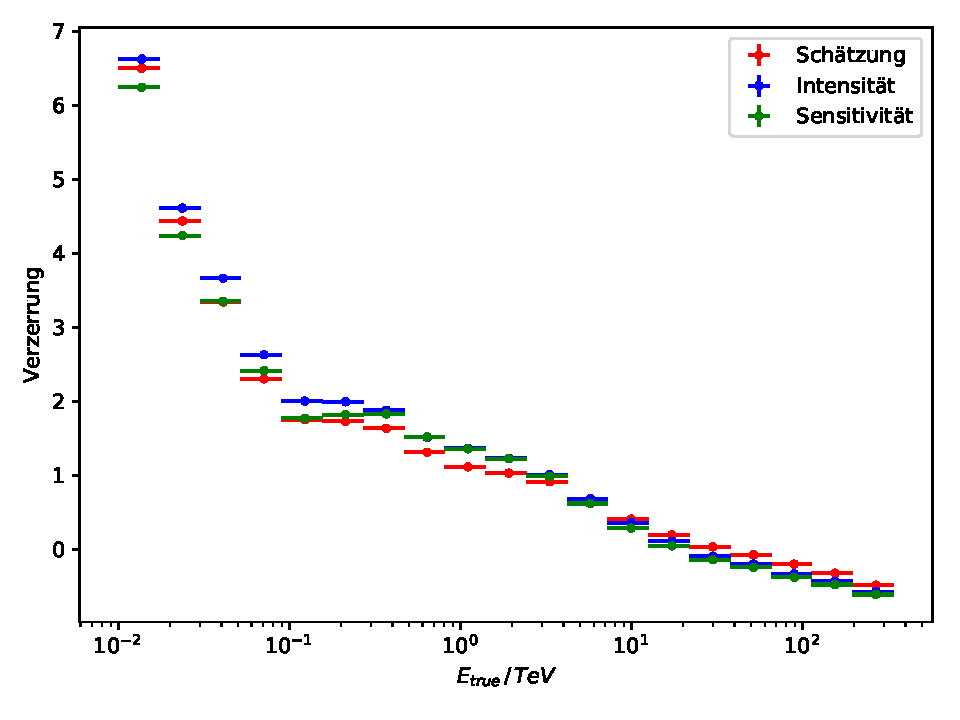
\includegraphics[width=0.7\textwidth]{Plots/RF_weights_bias.pdf}
  \centering
  \caption{Darstellung der Verzerrung für die arithmetische Mittelung, den Median und für eine gewichtete Mittelung mit der Intensität
            oder der Sensitivität als Gewicht.}
  \label{abb:w_bias}
\end{figure}
\begin{figure}
  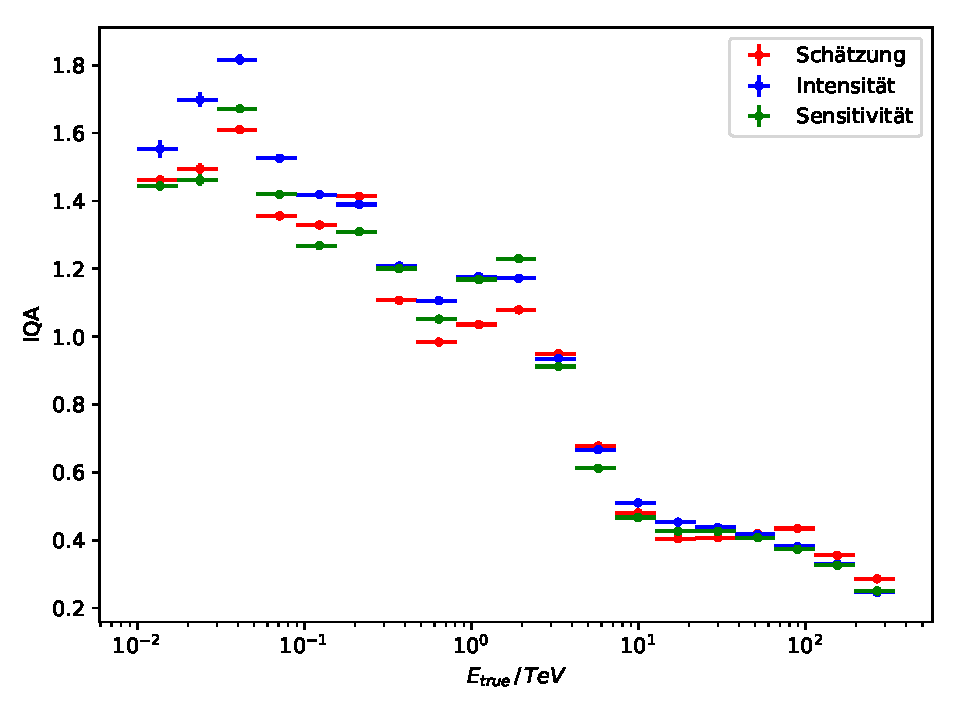
\includegraphics[width=0.7\textwidth]{Plots/RF_weights_resolution.pdf}
  \centering
  \caption{Auftragen des IQA des relativen Fehlers für verschiedene Energiebereiche, jeweils für den arithmetischen Mittelwert, den Median und
            für die mit der Intensität oder der Sensitivität gewichtet gemittelten Vorhersage.}
  \label{abb:w_IQA}
\end{figure}

Das Gewichten führt auf eine Energieschätzung, die in \autoref{abb:w_bias} und \autoref{abb:w_IQA} zu sehen ist.
Beide Gewichte führen nicht auf das gewünschte Ergebnis, wobei die Gewichtung mit der Intensität auf eine Verschlechterung der Qualität führt.
Die Sensitivität scheint zwar ein Indikator für die Sichtbarkeit zu sein, jedoch scheint die Höhe der Gewichtung nicht ausreichend zu sein, um
die Fehlschätzungen ausreichend zu korrigieren.
Durch die Energieabhängigkeit der Intensität scheint dieses Attribut als Gewicht ungeeignet zu sein.
Jedoch verbessert sich der gemittelte quadratische Fehler auf $\SI{58.68}{\tera\eV\squared}$ im Vergleich zu der Gewichtung mit der Sensitivität, wo er bei
$\SI{64.72}{\tera\eV\squared}$ bleibt.

Welche der Methoden die bessere Qualität liefert, hängt von der Analyse ab.
Soll ein Energiespektrum untersucht werden, wird Wert auf einen geringen relativen Fehler gelegt, was das Nutzen des Medians nahe legt.
Werden jedoch Linienspektren untersucht, kann der Mittelwert in einigen Energiebereichen die richtige Wahl sein, da dieser auf einen geringeren
absoluten Fehler führt.
Der Median sorgt für eine Verbesserung in niedrigen Energiebereichen, jedoch führt er zu einer Verschlechterung bei Energien von $(\num{1}-\num{10})\,\si{\tera\eV}$.
In diesem Bereich besitzt CTA jedoch die größte Statistik, womit der Qualitätsgewinn infrage gestellt wird, was durch den
gleichbleibenden gemittelten quadratischen Fehler bestätigt wird.

%Einfacher Mittelwert über gleiches Event; Nutzung von unterschiedlichen Gewichten;

\section{Verschachtelung von Regressionsverfahren}
\label{sec:nest}

Schon die Wichtigkeit der eventspezifischen Attribute in \autoref{abb:first_FI} deutet darauf hin, dass die zusammengefassten Attribute eines Ereignisses
mehr Information beinhalten, als die teleskopspezifischen Attribute.
Daher wird nach der ersten Schätzung ein zweiter Random Forest trainiert, der mithilfe von eventspezifischen Attributen Schätzungen für jedes Ereignis abgibt.
Zu den Attributen gehören die Anzahl der ausgelösten Teleskope sowie SST, MST und LST, die totale Intensität, die arithmetisch gemittelte Schätzung des
ersten Waldes, die Mittelwerte und Standardabweichungen der skalierten Größen und die Mittelwerte, Standardabweichungen, Maximal- und Minimalwerte der
Schätzungen von den SST, MST und LST.
\begin{figure}
  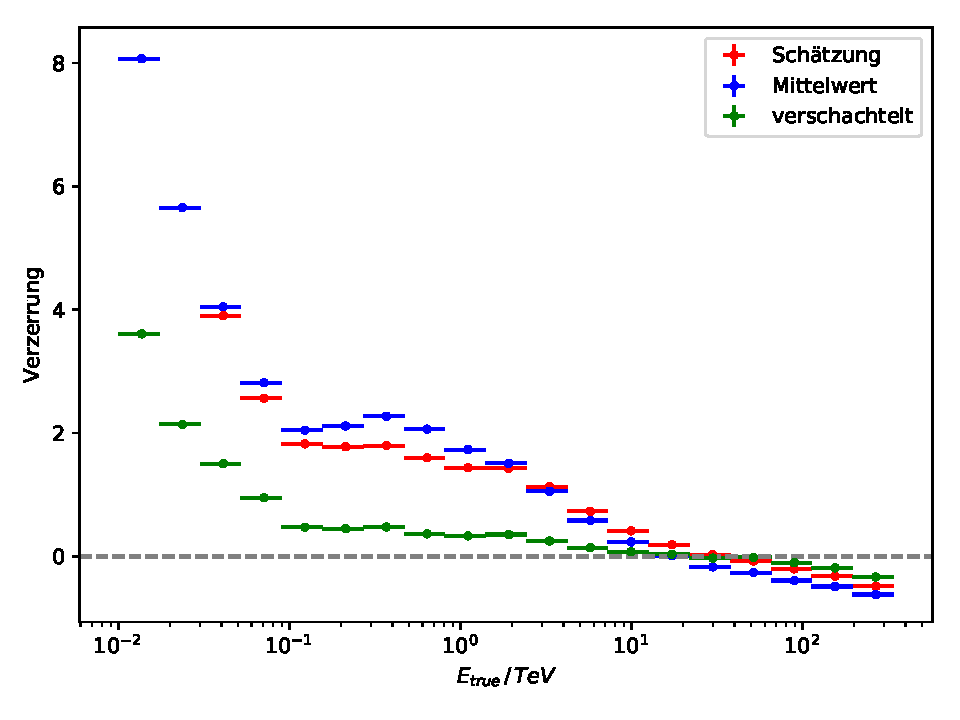
\includegraphics[width=0.7\textwidth]{Plots/RF_nested_bias.pdf}
  \centering
  \caption{Abbildung der Verzerrung nach einer Verschachtelung von zwei Random Forests. Es ist eine deutliche Verbesserung gegenüber der Mittelwertbildung
            zu erkennen.}
  \label{abb:nest_bias}
\end{figure}
\begin{figure}
  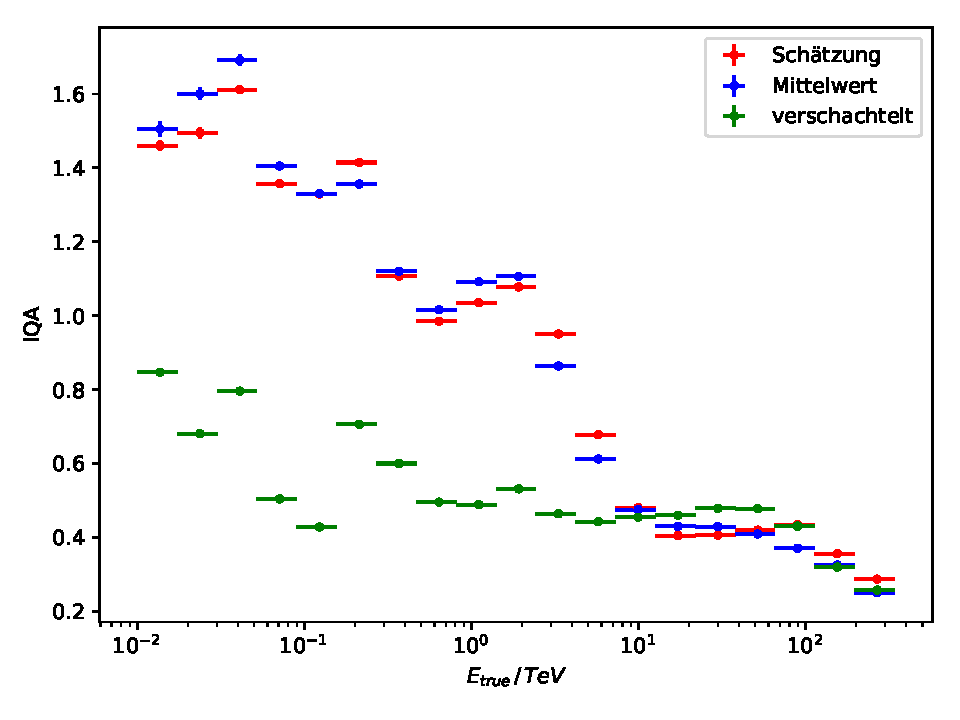
\includegraphics[width=0.7\textwidth]{Plots/RF_nested_resolution.pdf}
  \centering
  \caption{Abbildung des IQA für den zweiten Random Forest. Die Verschachtelung führt auf eine starke Verringerung des IQA bei niedrigen Energien.}
  \label{abb:nest_IQA}
\end{figure}

Der Random Forest wird mit $\num{498081}$ Ereignissen trainiert und getestet.
In \autoref{abb:nest_bias} und \autoref{abb:nest_IQA} ist die Qualität des zweiten Schätzers dargestellt und der gemittelte quadrierte Fehler fällt
auf $\SI{37.18}{\tera\eV\squared}$.
Die Verschachtelung der Entscheidungswälder führt auf eine verbesserte Qualität in allen Energiebereichen, sowohl bei der Verzerrung als auch bei dem IQA,
wodurch ein Übertraining durch den zweiten Wald ausgeschlossen werden kann.

Die genutzten Attribute haben eine starke Korrelation aufgrund der Gewinnung der Attribute aus der gleichen Information.
Dies ist durch die Anzahl an Ausreißer in \autoref{abb:second_FI} zu erkennen.
\begin{figure}
  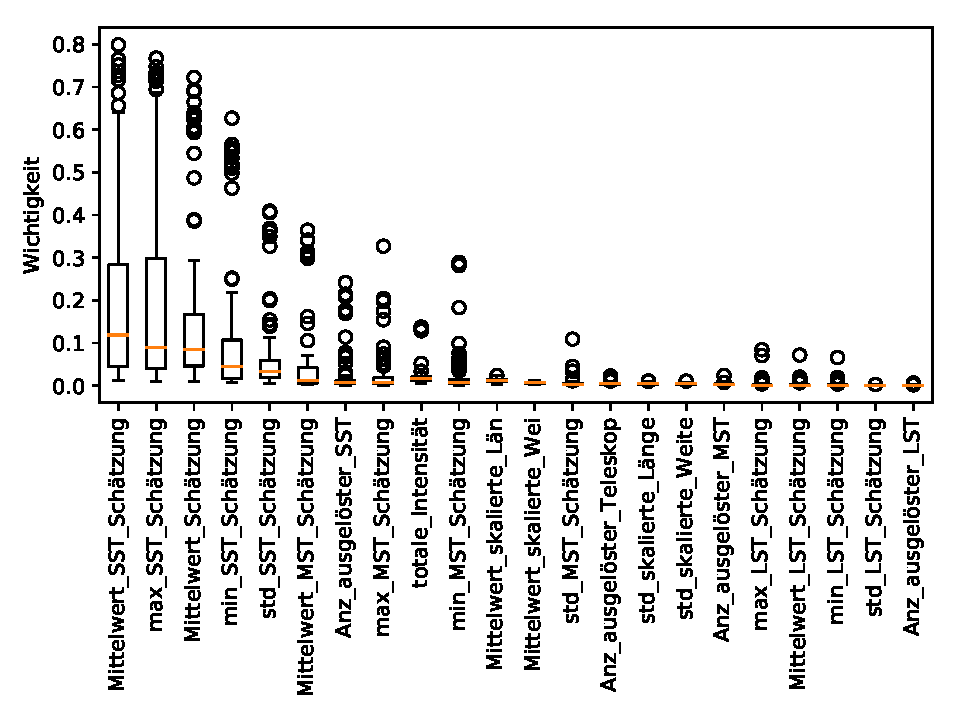
\includegraphics[width=0.7\textwidth]{Plots/feautureimportance_boxplot_secondForest.pdf}
  \centering
  \caption{Abbildung der Wichtigkeit der Attribute im zweiten Random Forest. Die Informationen der SST und die
          Schätzung des ersten Random Forest sind bedeutende Attribute und die hohe Fluktuation deutet auf eine
          Korreliertheit der Attribute hin.}
  \label{abb:second_FI}
\end{figure}
Eine genauere Untersuchung des Aufbaus der Entscheidungsbäume ergibt, dass die erste Separation der Datensätze häufig mithilfe der gemittelten Schätzung geschieht,
um sich in den Unterbäumen auf die für diesen Energiebereich interessanten Attribute zu konzentrieren.
Die Anzahl der ausgelösten SST stellt zum Beispiel einen guten Parameter für hohe Energien dar, da solche Photonen große Schauer erzeugen, die
zu großen Cherenkov-Kegeln führen.
Eine geringe Anzahl an ausgelösten SST stellt jedoch kein Kriterium für eine niedrige Photonenenergie dar, weil auch die Möglichkeit besteht, dass nur der
Rand des Schauers beobachtet wird.

Um die Frage zu beantworten, wie der Qualitätsgewinn im Vergleich zum Zeitaufwand steht, wird zunächst die Komplexität für das Ausbauen des Entscheidungswaldes untersucht,
welche im Mittel bei
\begin{equation}
  \Theta (MK\tilde{N} \log^2\left(\tilde{N}\right))
\end{equation}
liegt~\cite[96]{understanding_RF}.
Dies gilt für Random Forests mit $M$ Bäumen, die mit $K$ zufällig gezogenen Attributen und $N$ Datenpunkten vollständig ausgebaut werden.
Da das Bootstrapping in \textsc{scikit-learn} Datensätze erzeugt, die gleich groß wie der Originaldatensatz sind, gilt $\tilde{N}= N$.
Der Datensatz des zweiten Entscheidungswaldes besitzt $N_2 \approx \frac{1}{5}N_1$ Datenpunkte, da im Mittel $\approx 5$ Teleskope auslösen.
Damit stellt
\begin{equation}
  \Theta \left(MK\frac{1}{5}\tilde{N_1} \log^2\left(\frac{1}{5}\tilde{N_1}\right)\right)
\end{equation}
den zusätzlichen Zeitaufwand dar.
Da der Zeitaufwand der Schätzung, welcher
\begin{equation}
  \Theta\left(M\log\left(\frac{1}{5}N\right)\right)
\end{equation}
beträgt~\cite[98]{understanding_RF}, für die angestrebte Echtzeitanalyse von größerem Interesse ist, steht der Qualitätsgewinn noch besser da.
Außerdem werden die Entscheidungsbäume nicht vollständig ausgebaut, wodurch der Zeitaufwand deutlich verringert wird, jedoch können beide Entscheidungswälder nicht
parallelisiert werden, wodurch definitiv ein Zeitverlust entsteht.

\section{Transformation der Energie}

In \autoref{abb:Energie_RF} ist ein Abschneiden für niedrige Energien durch den Schätzer zu beobachten.
Durch die logarithmische Skala scheint es ein drastischer Schnitt zu sein, jedoch ist der Fehler, der entsteht, wenn alle Energien $E_\gamma < \SI{0.1}{\tera\eV}$
auf $\SI{0.1}{\tera\eV}$ geschätzt werden, gering.
Daher konzentriert sich der Algorithmus darauf, die großen Energien richtig zu schätzen.
Dies führt jedoch auf einen großen relativen Fehler für kleine Energien, wie er in \autoref{abb:mean_median_bias} zu sehen ist und somit auf eine schlechte
Energieauflösung.

Eine bijektive Transformation auf $\symbb{R}^+$ mit
\begin{equation}
  E_{\symup{trafo}}=\ln(E_\gamma +3)
  \label{eqn:trafo}
\end{equation}
führt auf eine kleinere Zielmenge des Schätzers, wodurch die Qualität weniger stark energieabhängig ist.
Eine anschließende Rücktransformation mit
\begin{equation}
  E_\gamma = \exp \left(E_{\symup{trafo}}\right)-3
\end{equation}
führt wieder auf die richtige Energie.
\begin{figure}
  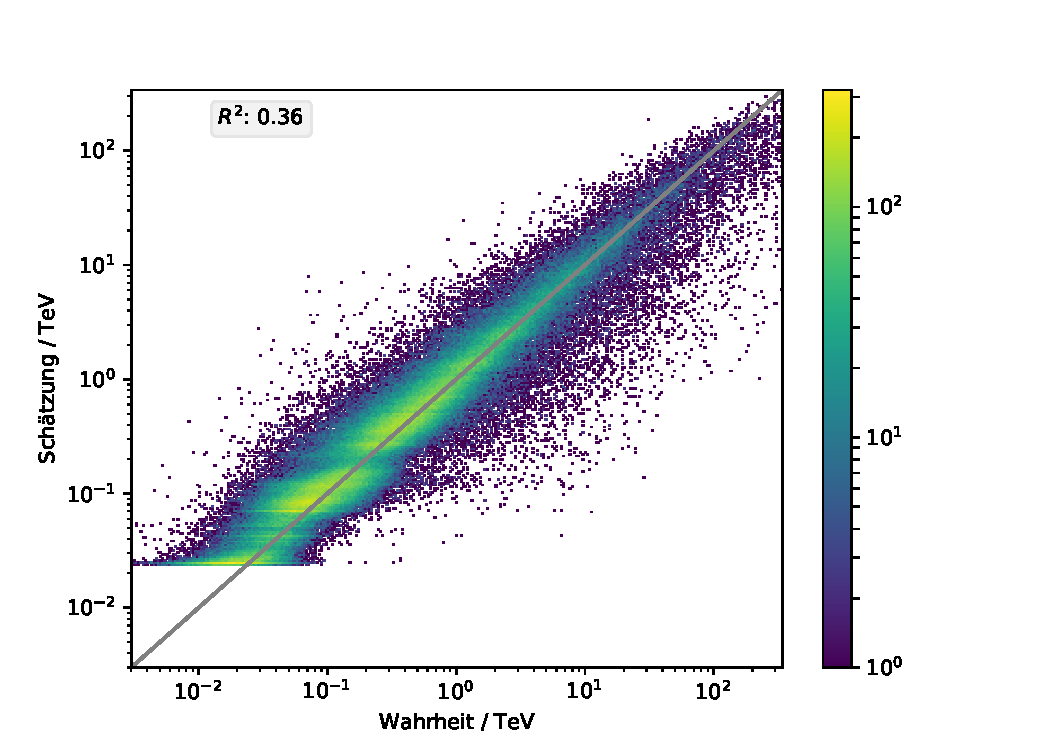
\includegraphics[width=0.7\textwidth]{Plots/trafo_encaps.pdf}
  \centering
  \caption{Abbildung der geschätzten Energie durch einen auf die transformierte Energie trainierten Random Forest. Der Schätzer schneidet fast eine Größenordnung
          später ab als der Schätzer aus \autoref{sec:first}.}
  \label{abb:Energie_trafo}
\end{figure}

Es wird das verschachtelte Modell aus \autoref{sec:nest} benutzt, wobei beide Schätzer auf die transformierte Energie trainiert werden.
\autoref{abb:Energie_trafo} zeigt, dass der Schätzer beinahe eine Größenordnung später abschneidet und die Transformation keinen Genauigkeitsverlust
in anderen Energiebereichen zufolge hat.
Der Schätzer scheint mehr Wert auf einen geringen Fehler bei kleinen Energien zu legen.
Schon das Verschachteln der Algorithmen sorgt für ein Herabsetzen der Grenze, da durch das frühe Trennen der Energiebereiche im Entscheidungsbaum, dem
Algorithmus die Möglichkeit gegeben wird, sich auf die Verbesserung der niedrigen Energiebereiche zu konzentrieren.
Die Deutung von \autoref{abb:trafo_bias} und \autoref{abb:trafo_IQA} zeigt, dass die Transformation die Qualität im Vergleich
zum Algorithmus aus \ref{sec:nest} verbessert.
\begin{figure}
  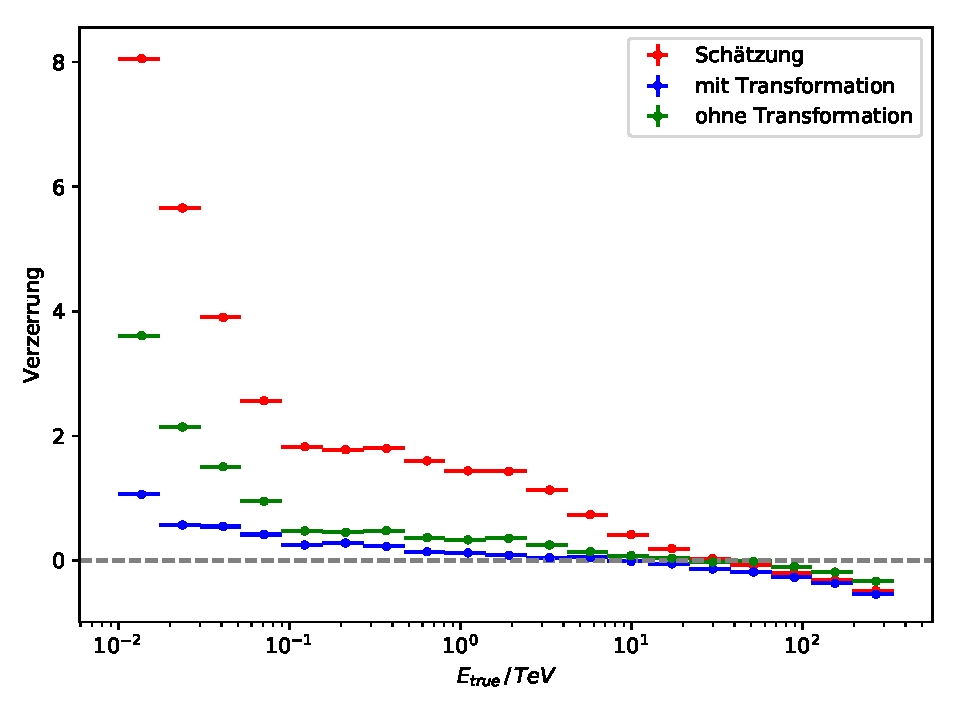
\includegraphics[width=0.7\textwidth]{Plots/trafo_nested_bias.pdf}
  \centering
  \caption{Darstellung der Verzerrung bei einer verschachtelten Schätzung mit und ohne Transformation der Art \eqref{eqn:trafo} sowie die Mittelwertbildung ohne Transformation. Die Transformation führt zu einer Verringerung
          des relativen Fehlers in niedrigen Energiebereichen.}
  \label{abb:trafo_bias}
\end{figure}
\begin{figure}
  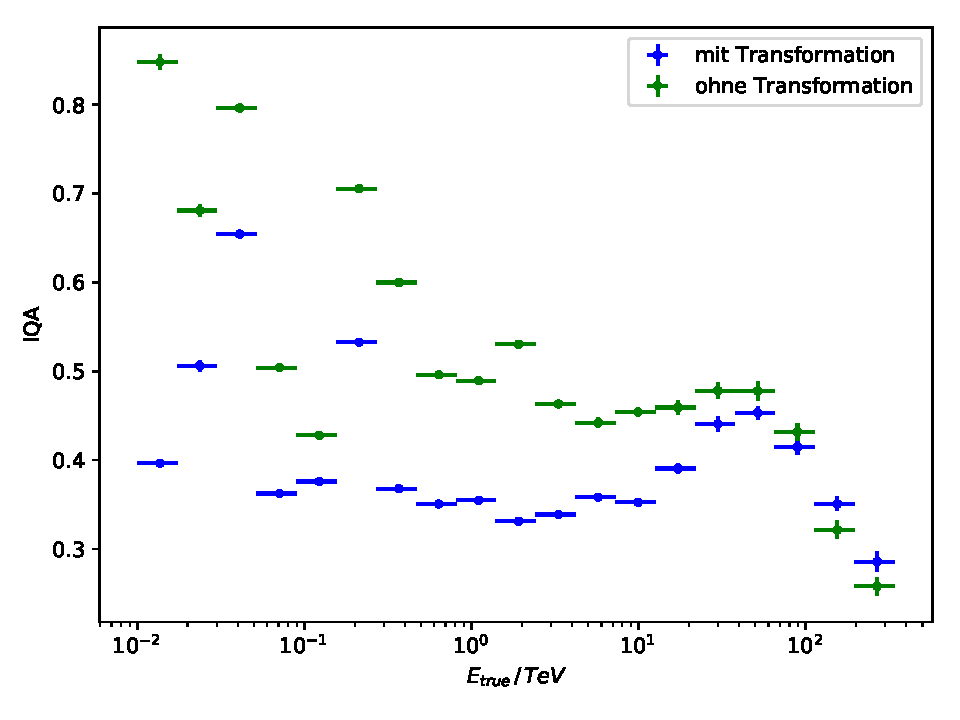
\includegraphics[width=0.7\textwidth]{Plots/trafo_nested_resolution.pdf}
  \centering
  \caption{Abbildung der Energieauflösung nach einer Transformation des Zielbereichs im Vergleich zu der untransformierten gemittelten Schätzung und der verschachtelten Schätzung. Die Transformation führt auf eine
          Verbesserung in niedrigen Energiebereichen.}
  \label{abb:trafo_IQA}
\end{figure}
Sowohl der IQA als auch die Verzerrung des relativen Fehlers werden mithilfe der Transformation bei niedrigen Energien geringer.
Bei $E_\gamma > \SI{30}{\tera\eV}$ muss jedoch eine Verschlechterung der Verzerrung und Auflösung in Kauf genommen werden, welche jedoch eine große Verschlechterung
bezogen auf den absoluten Fehler bedeutet, der von $\SI{37.18}{\tera\eV\squared}$ auf $\SI{53.65}{\tera\eV\squared}$ steigt.

\chapter{Zusammenfassung und Ausblick}

\section{Fazit der Arbeit}

%deutliche verbesserung bei Verschachtelung und mean scaled values;

\section{Perspektiven}

% versuch neue mean scaled Values zu definieren; bessere Transformation finden;


\appendix
% Hier beginnt der Anhang, nummeriert in lateinischen Buchstaben
\chapter{Ein Anhangskapitel}


\backmatter
\printbibliography

\cleardoublepage
\thispagestyle{empty}
\section*{Eidesstattliche Versicherung}
Ich versichere hiermit an Eides statt, dass ich die vorliegende Abschlussarbeit mit dem Titel \enquote{\thetitle} selbstständig und ohne unzulässige fremde Hilfe erbracht habe.
Ich habe keine anderen als die angegebenen Quellen und Hilfsmittel benutzt, sowie wörtliche und sinngemäße Zitate kenntlich gemacht. 
Die Arbeit hat in gleicher oder ähnlicher Form noch keiner Prüfungsbehörde vorgelegen.

\vspace*{1cm}\noindent
\begin{center}
  \begin{tabular}{@{}p{0.4\textwidth}@{\hspace{0.15\textwidth}}p{0.4\textwidth}@{}}
  \rule{\linewidth}{0.25pt}& \rule{\linewidth}{0.25pt}\\
  Ort, Datum & Unterschrift
  \end{tabular}
\end{center}

\subsection*{Belehrung}
Wer vorsätzlich gegen eine die Täuschung über Prüfungsleistungen betreffende Regelung einer Hochschulprüfungsordnung verstößt, handelt ordnungswidrig.
Die Ordnungswidrigkeit kann mit einer Geldbuße von bis zu \SI[round-mode=places, round-precision=2]{50000}{€} geahndet werden. 
Zuständige Verwaltungsbehörde für die Verfolgung und Ahndung von Ordnungswidrigkeiten ist der Kanzler/die Kanzlerin der Technischen Universität Dortmund. 
Im Falle eines mehrfachen oder sonstigen schwerwiegenden Täuschungsversuches kann der Prüfling zudem exmatrikuliert werden \mbox{(\S\,63 Abs. 5 Hochschulgesetz --HG--).}

Die Abgabe einer falschen Versicherung an Eides statt wird mit Freiheitsstrafe bis zu 3 Jahren oder mit Geldstrafe bestraft.

Die Technische Universität Dortmund wird ggf.\ elektronische Vergleichswerkzeuge (wie z.\,B.\ die Software \enquote{turnitin}) zur Überprüfung von Ordnungswidrigkeiten in Prüfungsverfahren nutzen. \\[\baselineskip]

\noindent Die oben stehende Belehrung habe ich zur Kenntnis genommen.\\[1cm]
\begin{center}
\begin{tabular}{@{}p{0.4\textwidth}@{\hspace{0.15\textwidth}}p{0.4\textwidth}@{}}
\rule{\linewidth}{0.25pt}& \rule{\linewidth}{0.25pt}\\
Ort, Datum & Unterschrift
\end{tabular}
\end{center}

\end{document}
